%niveau estimé : 4ème
    %date de projection : 18_10_2024
    %themes abordés : Pourcentage, Diviseurs, Addition
    
    \vspace{-0.5cm}
    \begin{multicols}{2}
        \boiteQFQ{Question 1 :}{
            Un article coûte $22{,}50\,\text{\euro{}}$ et subit une \textbf{augmentation} de $25\%$ de son prix.\\ \textbf{Calculer} le nouveau prix de l'article.
        }
        \boiteQFQ{Question 2 :}{
            \textbf{Déterminer} tous les \textbf{diviseurs} du nombre $68$.
        }
    \end{multicols}
    \vspace{-0.85cm}
    \begin{multicols}{2}
        
        \boiteQFQ{Question 3 :}{
            \textbf{Calcule} la somme des fractions suivantes : \[\dfrac{3}{7} + \dfrac{5}{9}\]
        }
        \boiteQFA{}
    \end{multicols}
    
    \newpage
    \vspace{-0.5cm}
    \begin{multicols}{2}
        \boiteQFQ{Question 1 :}{
            Un article coûte $22{,}50\,\text{\euro{}}$ et subit une \textbf{augmentation} de $25\%$ de son prix.\\ \textbf{Calculer} le nouveau prix de l'article.
        }
        \boiteQFQ{Question 2 :}{
            \textbf{Déterminer} tous les \textbf{diviseurs} du nombre $68$.
        }
        
    \end{multicols}
    \vspace{-0.85cm}
    \begin{multicols}{2}
        
        \boiteQFQ{Question 3 :}{
            \textbf{Calcule} la somme des fractions suivantes : \[\dfrac{3}{7} + \dfrac{5}{9}\]
        }
        \boiteQFA{
            \vspace{-0.35cm}
            \begin{itemize}[itemsep=0.2em]
                \item[\raisebox{-0.2cm}{\begin{itembox} \textbf{Q.1} \end{itembox}}] \def\newprice{\num{\fpeval{22.50*0.25}}}
                $28{,}13 \text{\euro{}}\,$
            \end{itemize}
        }
    \end{multicols}
    \newpage
    \vspace{-0.5cm}
    \begin{multicols}{2}
        \boiteQFQ{Question 1 :}{
            Un article coûte $22{,}50\,\text{\euro{}}$ et subit une \textbf{augmentation} de $25\%$ de son prix.\\ \textbf{Calculer} le nouveau prix de l'article.
        }
        \boiteQFQ{Question 2 :}{
            \textbf{Déterminer} tous les \textbf{diviseurs} du nombre $68$.
        }
        
    \end{multicols}
    \vspace{-0.85cm}
    \begin{multicols}{2}
        
        \boiteQFQ{Question 3 :}{
            \textbf{Calcule} la somme des fractions suivantes : \[\dfrac{3}{7} + \dfrac{5}{9}\]
        }
        \boiteQFA{
            \vspace{-0.35cm}
            \begin{itemize}[itemsep=0.2em]
                \item[\raisebox{-0.2cm}{\begin{itembox} \textbf{Q.1} \end{itembox}}] \def\newprice{\num{\fpeval{22.50*0.25}}}
                $28{,}13 \text{\euro{}}\,$
                \item[\raisebox{-0.2cm}{\begin{itembox} \textbf{Q.2} \end{itembox}}] $1, \, 2, \, 4, \, 17, \, 34, \, 68$
            \end{itemize}
        }
    \end{multicols}
    \newpage
    
    \begin{multicols}{2}
        \boiteQFQ{Question 1 :}{
            Un article coûte $22{,}50\,\text{\euro{}}$ et subit une \textbf{augmentation} de $25\%$ de son prix.\\ \textbf{Calculer} le nouveau prix de l'article.
        }
        \boiteQFQ{Question 2 :}{
            \textbf{Déterminer} tous les \textbf{diviseurs} du nombre $68$.
        }
        
    \end{multicols}
    \vspace{-0.85cm}
    \begin{multicols}{2}
        
        \boiteQFQ{Question 3 :}{
            \textbf{Calcule} la somme des fractions suivantes : \[\dfrac{3}{7} + \dfrac{5}{9}\]
        }
        \boiteQFA{
            \vspace{-0.35cm}
            \begin{itemize}[itemsep=0.2em]
                \item[\raisebox{-0.2cm}{\begin{itembox} \textbf{Q.1} \end{itembox}}] \def\newprice{\num{\fpeval{22.50*0.25}}}
                $28{,}13 \text{\euro{}}\,$
                \item[\raisebox{-0.2cm}{\begin{itembox} \textbf{Q.2} \end{itembox}}] $1, \, 2, \, 4, \, 17, \, 34, \, 68$
                \item[\raisebox{-0.2cm}{\begin{itembox} \textbf{Q.3} \end{itembox}}] $\dfrac{62}{63}$
            \end{itemize}
        }
    \end{multicols}
    
    \newpage
    
    %\begin{multicols}{2}
    \boiteQFdet{Question 1 :}{
        
        Un article coûte $22{,}50\,\text{\euro{}}$ et subit une \textbf{augmentation} de $25\%$ de son prix.\\ \textbf{Calculer} le nouveau prix de l'article.
        
        \tikz{\draw[dashed, line width=1pt] (0,0) -- (\linewidth,0);}
        
        \vspace{-0.25cm}\begin{multicols}{2}
        
        
        Pour \textbf{calculer} le nouveau prix de l'article après une \textbf{augmentation} de $25\%$, on calcule le prix de l'augmentation :
        
        Augmentation $=\text{Prix initial} \times 25 \div 100$\\
        
        \def\augm{\num{\fpeval{22.50*0.25}}}
        
        \def\newprice{\num{\fpeval{22.50*1.25}}}
        
        Augmentation $= 22{,}50 \times 25 \div 100 =\augm $
        
        \columnbreak
        
        On peut donc calculer le nouveau prix de l'article :
        
        $ \text{Nouveau prix} = \text{Ancien prix} + \text{Augmentation}$
        
        Nouveau prix $= 22{,}50 + \augm = \newprice$
        
        Ainsi, le \textbf{nouveau prix} de l'article est $ 28{,}13\text{\euro{}}$ ( arrondi aux centièmes ).
        
    \end{multicols}
}

\newpage

\boiteQFdet{Question 2 :}{
    
    \textbf{Déterminer} tous les \textbf{diviseurs} du nombre $68$.
    
    \tikz{\draw[dashed, line width=1pt] (0,0) -- (\linewidth,0);}
    
    
    \vspace{-0.25cm}\begin{multicols}{2}
    
    \textbf{Calcul des Diviseurs:}
    
    On repère les diviseurs de 68 en utilisant la méthode de recherche suivante :\\
    
    \begin{center}
        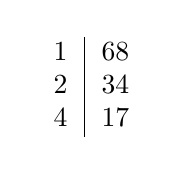
\begin{tikzpicture}
            \node at (0, 0) {
                \begin{tabular}{r|l}
                    1 & 68 \\
                    2 & 34 \\
                    4 & 17 \\
                \end{tabular}
            };
        \end{tikzpicture}
    \end{center}
    
    $68$ a donc $6$ \textbf{diviseurs :} $1, 2, 4, 17, 34,$ et $68$.
    
\end{multicols}
}

%\columnbreak
\newpage

\boiteQFdet{Question 3 :}{

\textbf{Calcule} la somme des fractions suivantes : \[\dfrac{3}{7} + \dfrac{5}{9}\]

\tikz{\draw[dashed, line width=1pt] (0,0) -- (\linewidth,0);}

\vspace{-0.25cm}\begin{multicols}{2}

Pour \textbf{calculer} la somme des deux \textbf{fractions} $\dfrac{3}{7} + \dfrac{5}{9}$, nous devons d'abord les mettre sur un \textbf{dénominateur commun}.

Le \textbf{plus petit dénominateur commun} des dénominateurs $7$ et $9$ est $63$. Donc, nous convertissons chaque fraction pour avoir ce même dénominateur :

\[
    \dfrac{3}{7} = \dfrac{3 \times 9}{7 \times 9} = \dfrac{27}{63}
\]
\[
    \dfrac{5}{9} = \dfrac{5 \times 7}{9 \times 7} = \dfrac{35}{63}
\]

Ensuite, nous \textbf{additionnons} ces nouvelles fractions par leurs numérateurs :

\[
    \dfrac{27}{63} + \dfrac{35}{63} = \dfrac{27 + 35}{63} = \dfrac{62}{63}
\]

Par conséquent, la somme des fractions est \(\boxed{\dfrac{62}{63}}\).

\end{multicols}
}
%\end{multicols}